\section{Routing Algorithms and IoT Based Evacuation Management}
\label{sec:pastwork:Routing Algorithms and IoT Based Evacuation Management}

Routing algorithms and maze solving algorithms have especially been applied to the structural domains for the real time analysis of shortest paths and obstacle avoidance by both machine and human agents since the time the earliest shortest paths algorithms were developed. The development of the shortest path algorithm by Dijkstra in 1956, especially has seen a plethora of applications in various fields. As one can guess most of its applications have been catered to graph based problems and obstacle avoidance. Shortest paths exit strategy formation approach is a good way to analyse a safe egress as it provides obstacle avoidance as well. How can it successfully be applied to a real disaster scenario? Before the advancements were made to IoT based infrastructure, maze solving algorithms were used to successfully analyze a safe egress. 

IoT and computation systems have brough about a tremendous potential to perceive the environment and then form the necessary strategies that are required to safely escort the human agents to a safe exit point during the time of disaster. Modern evacuation systems have sensors in place to allow for better perception of the world during a disaster scenario. For instance the work by Kobes et al. determined that during fire related disaster scenarios, 56.3\% of the participating agents were able to determine the exit points based on the exit signs when there was no smoke present whilst 81.8\% was able to identify exit points only based on the exit signs when their vision was imparied due to smoke [11]. Based on such data for instance, it greatly enhances our need to analyse the fastest and shortest egress path so that all human agents in the vicinity can get to the exit points. The shortest path algorithm - Dijkstra's algorithm is currently used as a great tool to provide the shortest exit points as it is demonstrated in the work by Jehyun Cho [12]. His research pertains to the dynamic analysis of a shortest path algorithm based on information obtained from the sensors and the smart infrastructure.  

In order to address the issue of agent(s) and infrastructure mapping during a disaster event, state of the art sensors are placed all through the infrastructure in order to perceive the environment and the surrounding structures in order to analyze a safe egress. Motion detectors for instance are used to understand how many people are still trapped inside the building during a catastrophe. One example of using IoT technologies is proposed by Prasad Annadata et al. using multiple WIFI channels and the aforementioned motion detectors [13]. Based on the statistics gathered heuristic solutions are proposed in order to detect the number of personnel inside the infrastructure as well as perceive the environment. 

Although the proposed methods and techniques are helpful in determining the shortest path to an exit point, they rarely can be used in a realistic scenario due to its simplistic nature. A real world scenario is more complex due the social dynamics of people. Such complexities are better understood while simulating agents in real and static simulations and then performing an analysis based on the observed stats. Such is what I hope to achieve through this thesis.

Existing literature on surveying personnel and the surrounding infrastructure for assistance based support for immediate first responders include the work the done by Palmieri et al., who proposes a hybrid cloud architecture to manage and store the necessary required resources to command and control activities during emergencies [14]. However the work done by H. Muccini et al. [5] aims to improve this work by adapting geolocation of first responders to track people during a disaster for evacuation. Furthermore W.Choi et al. [15] proposes to model building evacuation by dynamic flow maximization and by considering variable capacities on some arcs as a function of flows in incident arcs. For the purposes of modeling our topology we have used a similar arc based geometry for determining the topological capacity of a particular cell into which the entire infrastructure is divided into. Chen et al. [16] in addition to the above, proposes a flow control algorithm that calculates evacuation paths depending on building plan and total number of
evacuees. Computation in this case aims at minimizing total evacuation time and assigning an optimal number of evacuees to each evacuation path. However [5] provides a robust solution by architecting an IoT system to monitor and update dynamically the topology of the environment.

Another important aspect that remains unaddressed is that in real disaster scenarios, over crowding and congestion of certain pathways and exit points are bound to occur frequently. The issue of congestion is serious and perilous and is arguably pointed out by a case study performed by John El Khoury [17] and analyses the dangers due to high traffic intensity during a disaster event. Although the analysis is performed on a wide scale city range, the implications of congestion and other such constraints are just a applicant to a much smaller scale infrastructure. To dynamically reallocate personnel to routes that are not just shortest paths but optimal paths is what we try to achieve through these simulations and added constraints. The work done by Antoine Desmet et al. [18] addresses the congestion issue by a "self adaptation" algorithm much inspired by the computer network routing algorithm - The Cognitive Packet routing algorithm by E. Gelenbe [19]. A robust evacuation with optimized routing solution proposed by H.Muccini et al. [5] are as follows:

\begin{itemize}
  \item Optimal solutions that can be continuously updated, so evacuation guidelines can be adjusted according to visitors position that evolve over time.
  \item Paths that become suddenly unfeasible can automatically be discarded by the system.
  \item The model can be incorporated into a mobile app supporting emergency units to evacuate closed or open spaces.
\end{itemize} 

The aforementioned algorithm is still incomplete as dynamic and realistic constraints are yet to be added. The constraints are 4 fold as mentioned in the introduction section. Over the course of chapter 3, the details of the algorithm is explained and how these constraints provide an even more optimized route since it considers congestion, grouping, varying age and speeds in addition. 

% Everyone needs floating figures in their dissertation. 

% As shown in Figure~\ref{fig:pastwork:titlepage}, the Mudd Library dissertation requirements~\cite{muddthesis2009} specify additional options for formatting the title page. For example, if your thesis has multiple volumes, or to indicate the proper formatting for a master's thesis.

% \begin{figure}[htb]
%   \begin{center}
%     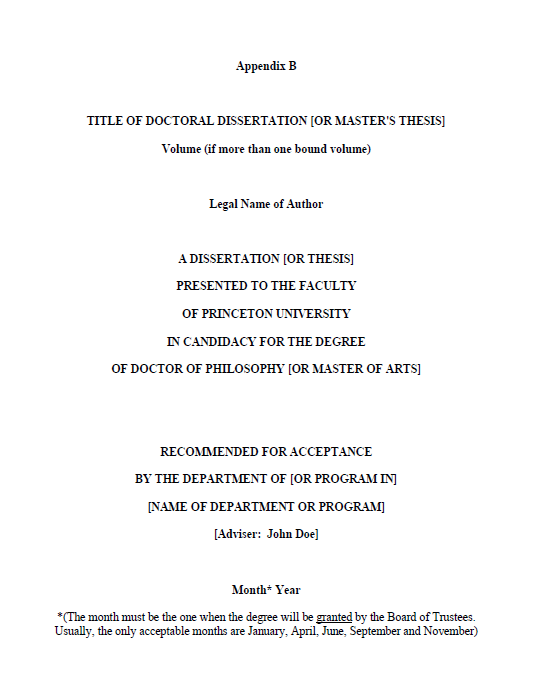
\includegraphics[width=0.9\linewidth]{ch-pastwork/figures/titlepage}
%     \caption[Sample Title Page Layout]{Sample title page layout~\cite{muddthesis2009}}
%     \label{fig:pastwork:titlepage}
%   \end{center}
% \end{figure}
